% Provenance (never printed): see sources/outline_sources.md (Year 3: elastic waves
% recalled from the physics books; rays in a spherical Earth; travel-time tables;
% surface waves and dispersion; normal modes, told; linear inverse problems and
% seismic tomography). Brief: sources/book5/BRIEFS.md, ch. 1. Curves from
% figdata/bachelor-3/ray_tracing.py, love_dispersion.py, tomo_checkerboard.py;
% exercise and problem values in the Book 5 scratch calculator calc/ch01.py.
\chapter{地震学与地球成像}\label{ch:b3:seismology-imaging}

1960 年 5 月 22 日，协调世界时 19:11，自 1900 年以来记录到的最大地震，
在智利南部近海破裂了俯冲带，震级 9.5。
% ledger: usgs5:chile1960
其 P 波约 20 分钟后到达地球另一侧的台站，
其面波数次绕行全球；此后数日，
长周期仪器记录到整个地球在振动，
周期接近一小时，像被敲响的钟。这些信号中的每一个都携带
关于其所穿越岩石的信息。由数百万个此类
波的到达时间（读自数千个台站），地震学家不仅建立了
下文回顾的地球分层模型，而且得到了地幔的三维图像，
其中下沉的板片与上升的地幔柱表现为
波速略快或略慢于平均值的区域。本章说明以下各点：
射线如何穿过球形地球，面波如何
借助频散探测地壳与地幔，整个行星的自由振动如何描述，
以及如何把数千个走时
通过求解线性\omterm{def:b3:seismology-imaging:inverse}{反演问题}转化为一幅图像。

\begin{recall}
在各向同性弹性固体中传播的体波有两种：P 波，
速度 $\alpha = \sqrt{(K + \tfrac43\mu)/\rho}$，S 波的速度为
$\beta = \sqrt{\mu/\rho}$，其中 $K$ 与 $\mu$ 分别为体积模量与剪切模量，
$\rho$ 为密度；S 波不能穿过液体（见物理书本科三年级分册的
连续介质弹性一章）。相速度随频率变化的波称为
色散波；其能量以群速度
$U = \mathrm d\omega/\mathrm dk$ 传播（见物理书本科二年级分册中关于
波动的一章）。有界弹性体在一组离散的
简正模式中自由振动（同一分册）。台站的震中距 $\Delta$ 是
地心处震中与台站之间的夹角；走时曲线
给出首达时间相对 $\Delta$ 的变化，地核
对直达 P 波形成影区（第 2 册，十一年级）。参考地球模型，
地震不连续面与首波已在本科一年级分册
其分层地球一章中已学过。最小二乘与高斯
误差定律则属于数学书的内容。
\end{recall}

\section{球形地球中的射线}

地震波前位于远离震源的介质中，且其性质
在一个波长内变化缓慢，可由射线追踪：射线即
处处与波前垂直的曲线，能量沿其传播。在
速度均匀的介质中，射线为直线；速度变化处，
射线按斯涅耳折射定律发生弯折。地球中的速度主要取决于
深度，故第一近似模型取为球对称：
所考虑的波（P 波或 S 波）的速度 $v(r)$ 仅是半径 $r$ 的函数。

\begin{theorem}[球形地球中的斯涅耳定律]\label{thm:b3:seismology-imaging:snell}
在波速为 $v(r)$ 的球对称地球中，设 $i$ 为
射线与该点处半径之间的夹角，该点处半径为 $r$。沿整条射线，
\[
  \frac{r\sin i}{v(r)} = p
\]
为常数。
\end{theorem}

\begin{proof}
将地球替换为薄的同心球壳，每层速度均匀。在一层球壳内
射线为直线；距球心为 $d$ 的直线
与半径为 $r$ 的球面相交，交角 $i$ 满足
$r\sin i = d$（由球心、垂足与该点组成的直角三角形），
故 $r\sin i$ 在该层顶部与底部
取值相同。在两层球壳的分界面（半径为 $r$）处，
速度分别为 $v_1$ 与 $v_2$，由斯涅耳定律得 $\sin i_1/v_1 = \sin i_2/v_2$，故
$r\sin i/v$ 在该处连续。在一层球壳内 $v$ 为常数，且
$r\sin i$ 为常数，故 $r\sin i/v$ 在该层内亦为常数。于是
沿整条射线为常数；令球壳厚度趋于
零，即得连续变化的 $v(r)$ 的结论。
\end{proof}

\begin{definition}[射线参数，转折点]\label{def:b3:seismology-imaging:ray-parameter}
在球对称地球中，射线的常数 $p = r\sin i/v(r)$ 称为
该射线的\emph{射线参数}\index{射线参数}，单位为秒每弧度。在
地表处 $p = R\sin i_0/v_0$，其中 $i_0$ 为出射角，$v_0$
为地表处的速度。射线水平的点（$i = \ang{90}$）
即其\emph{射线转折点}\index{射线转折点}，
位于半径 $r_t$ 处，满足
\[
  \frac{r_t}{v(r_t)} = p .
\]
射线在其下方重新上升，
关于过转折点的半径对称。
\end{definition}

记 $\eta(r) = r/v(r)$。参数为 $p$ 的射线只能存在于
$\eta \ge p$ 处，因为 $\sin i = p/\eta \le 1$。若 $\eta$ 随深度减小，
正如地幔大部分区域那样，每条射线都在 $\eta$
降至 $p$ 的深度处转折，出射更陡（$p$ 更小）的射线转折得更深。
若 $\eta$ 随深度\emph{增大}（因速度随深度急剧下降，
这在核幔边界处发生，那里 P 波速度由
13.7 降至 \qty{8.0}{km.s^{-1}}），% ledger: ak135:cmb
射线不能在此转折：射线被向下弯折，穿过该层后在远处射出。
此类跳跃在地表形成影区。

\begin{omfigure}
\begin{tikzpicture}[font=\small, x=1.6cm, y=1.6cm]
% concentric shells, centre O at (0,-9) (outside the picture); ray computed by
% Snell's law for v = 1, 1.35, 1.68 and a take-off angle of 30 deg
% (scratch calc/shells_fig.py)
\coordinate (O) at (0,-9);
\fill[blue!6] ($(O)+(62:9)$) arc (62:118:9) -- ($(O)+(118:8.4)$) arc (118:62:8.4) -- cycle;
\fill[blue!12] ($(O)+(62:8.4)$) arc (62:118:8.4) -- ($(O)+(118:7.8)$) arc (118:62:7.8) -- cycle;
\fill[blue!18] ($(O)+(62:7.8)$) arc (62:118:7.8) -- ($(O)+(118:7.0)$) arc (118:62:7.0) -- cycle;
\draw[thick] ($(O)+(62:9)$) arc (62:118:9);
\foreach \r in {8.4, 7.8} {\draw[gray] ($(O)+(62:\r)$) arc (62:118:\r);}
\draw[gray, densely dashed] ($(O)+(62:7.0)$) arc (62:118:7.0);
\node[anchor=east] at ($(O)+(118.3:9)$) {$R$};
\node[anchor=east, gray!60!black] at ($(O)+(118.3:8.4)$) {$r_1$};
\node[anchor=east, gray!60!black] at ($(O)+(118.3:7.8)$) {$r_2$};
\node[blue!60!black] at ($(O)+(64:8.7)$) {$v_0$};
\node[blue!60!black] at ($(O)+(64:8.1)$) {$v_1$};
\node[blue!60!black] at ($(O)+(64:7.4)$) {$v_2$};
\coordinate (A) at (-3.295,-0.625);
\coordinate (B) at (-2.746,-1.062);
\coordinate (C) at (-1.920,-1.440);
\coordinate (T) at (0,-1.440);
\coordinate (C') at (1.920,-1.440);
\coordinate (B') at (2.746,-1.062);
\coordinate (A') at (3.295,-0.625);
% radii at the source and at the first boundary, towards the centre
\draw[densely dashed] ($(A)!-0.04!(O)$) -- ($(A)!0.12!(O)$);
\draw[densely dashed] ($(B)!-0.04!(O)$) -- ($(B)!0.11!(O)$);
\draw[densely dashed] (T) -- (0,-2.15);
\draw[very thick, red!70!black] (A) -- (B) -- (C) -- (T) -- (C') -- (B') -- (A');
\pic[draw, angle radius=0.75cm, pic text={$i_0$}, angle eccentricity=1.4] {angle = O--A--B};
\pic[draw, angle radius=0.65cm, pic text={$i_1$}, angle eccentricity=1.45] {angle = O--B--C};
\fill (A) circle (2pt) node[above left=1pt] {震源};
\fill (A') circle (2pt) node[above right=1pt] {台站};
\fill[red!70!black] (T) circle (1.6pt);
\node[anchor=north west, red!70!black] at (0.05,-1.47) {转折点，$r_t/v_2 = p$};
\node[anchor=north, font=\scriptsize] at (0,-2.15) {指向球心 $O$};
\end{tikzpicture}

\par\smallskip{\small 一条射线穿过被划分为速度均匀壳层的球形地球
（示意图，不按比例）。在每一壳层内射线为直线；在每个
边界处按斯涅耳定律折射，速度向下增大时折射方向偏离
半径方向。量 $r\sin i/v$ 沿射线保持同一值 $p$，
射线在其转折点处水平，此处 $r/v = p$，并
随后对称地重新上升。}
\label{fig:b3:seismology-imaging:shells}
\end{omfigure}

\omterm{def:b3:seismology-imaging:ray-parameter}{射线参数}不只是射线的常数，它还可以从
走时曲线上读出。

\begin{theorem}[走时曲线的斜率]\label{thm:b3:seismology-imaging:benndorf}
设 $T(\Delta)$ 为一条射线自地表震源至地表
台站的走时，其震中距为 $\Delta$（以弧度计）。则
\[
  \frac{\mathrm dT}{\mathrm d\Delta} = p ,
\]
即到达 $\Delta$ 处射线的\omterm{def:b3:seismology-imaging:ray-parameter}{射线参数}。
\end{theorem}

\begin{proof}
考虑由同一震源发出的两条相邻射线，它们到达地表
分别在 $\Delta$ 与 $\Delta + \mathrm d\Delta$ 处，且两者与半径的夹角均为 $i_0$，
过第一点的波前与射线垂直；
第二条射线在穿过该波前后，仍需经过一个小直角三角形的一条边，
其斜边为沿地表的弧 $R\,\mathrm d\Delta$，
该边所对的角为 $i_0$：长度为
$R\,\mathrm d\Delta\,\sin i_0$，速度为 $v_0$，因此
$\mathrm dT = R\sin i_0\,\mathrm d\Delta/v_0 = p\,\mathrm d\Delta$。
\end{proof}

该定理是关系式 $\mathrm dT/\mathrm dx = 1/c$ 的球面形式，
即走时曲线的斜率与沿地表的视速度 $c$ 之间的
关系。函数 $T(p)$ 与 $\Delta(p)$ 可以写成
对速度剖面的积分。

\begin{proposition}[作为积分的走时与距离]\label{prop:b3:seismology-imaging:integrals}
设 $\eta = r/v(r)$ 随深度减小，参数为 $p$ 的射线
在 $r_t$ 处转折并到达
\[
  \Delta(p) = 2\int_{r_t}^{R}\frac{p\,\mathrm dr}{r\sqrt{\eta^2 - p^2}},
  \qquad
  T(p) = 2\int_{r_t}^{R}\frac{\eta^2\,\mathrm dr}{r\sqrt{\eta^2 - p^2}},
\]
且截距时间 $\tau(p) = T - p\Delta$ 为
$\tau(p) = 2\int_{r_t}^{R}\sqrt{\eta^2 - p^2}\,\mathrm dr/r$.
\end{proposition}

\begin{proof}
沿射线上长度为 $\mathrm ds$ 的一段，半径的变化为
$\mathrm dr = \cos i\,\mathrm ds$，球心角的变化量为
$\mathrm d\Delta = \sin i\,\mathrm ds/r$，故 $\mathrm d\Delta = \tan i\,\mathrm dr/r$。
由 $\sin i = p/\eta$，$\tan i = p/\sqrt{\eta^2 - p^2}$，得出
下行一半的第一个积分；上行一半同理。走时为
$\mathrm dT = \mathrm ds/v = \mathrm dr/(v\cos i)$，且 $1/v = \eta/r$，
$1/\cos i = \eta/\sqrt{\eta^2 - p^2}$。最后，$T - p\Delta$ 的被积函数为
$(\eta^2 - p^2)/(r\sqrt{\eta^2 - p^2})$.
\end{proof}

这些积分即由模型计算\omterm{def:b3:seismology-imaging:tables}{走时表}的方法。本章的射线追踪脚本
对 2 千米厚的壳层做同样的求和，壳层取自
参考模型 PREM， % ledger: data:prem
并用两种方式加以检验：一是在匀速球体中，射线为
弦，此时 $T = 2R\sin(\Delta/2)/v$ 精确成立（练习 5）；另一种则是
与\cref{thm:b3:seismology-imaging:benndorf}比较，脚本并不使用该定理。

\begin{omfigure}
\begin{tikzpicture}
\begin{axis}[axis equal image, hide axis, width=0.66\linewidth,
  xmin=-1500, xmax=6700, ymin=-6700, ymax=6700, clip=false]
\addplot[draw=none, fill=gray!8, domain=0:360, samples=181] ({6371*cos(x)},{6371*sin(x)});
\addplot[black, thick, domain=0:360, samples=181] ({6371*cos(x)},{6371*sin(x)});
\addplot[orange!70!black, fill=orange!12, domain=0:360, samples=181] ({3480*cos(x)},{3480*sin(x)});
\addplot[orange!80!black, fill=orange!35, domain=0:360, samples=121] ({1221.5*cos(x)},{1221.5*sin(x)});
\addplot[blue!70!black, unbounded coords=jump] table[x=x, y=y] {figdata/out/bachelor-3-ray_tracing-rays-mantle.dat};
\addplot[red!70!black, unbounded coords=jump] table[x=x, y=y] {figdata/out/bachelor-3-ray_tracing-rays-core.dat};
% shadow zone for direct P, from 98.5 deg to the caustic B at 143.8 deg
\addplot[gray!60!black, line width=3pt, opacity=0.5, domain=98.5:143.8, samples=40]
  ({6371*sin(x)},{6371*cos(x)});
\fill (axis cs:0,6371) circle (2.2pt);
\node[anchor=south] at (axis cs:0,6371) {\small 震源};
\node[anchor=west, font=\small] at (axis cs:{6371*sin(120)+150},{6371*cos(120)}) {影区};
\node[anchor=west, font=\scriptsize] at (axis cs:{6371*sin(98.5)+120},{6371*cos(98.5)}) {\ang{98.5}};
\node[anchor=west, font=\scriptsize] at (axis cs:{6371*sin(143.8)+120},{6371*cos(143.8)}) {\ang{143.8}};
\node[font=\scriptsize, orange!50!black] at (axis cs:-1450,1650) {外核};
\draw[orange!50!black, thin] (axis cs:-700,-500) -- (axis cs:-2500,-4300) node[anchor=north, font=\scriptsize] {内核};
\node[font=\scriptsize] at (axis cs:-3300,4200) {地幔};
\end{axis}
\end{tikzpicture}

\par\smallskip{\small 地表震源发出的 P 射线经参考模型
PREM 中追踪，以 2 千米厚的壳层计算，出射角从 \ang{2} 到 \ang{34}
（与竖直方向的夹角）。蓝色：在地幔中转折的射线，至多
到达 \ang{98.5}；由于速度随深度增大，它们向上弯曲，
靠近顶部的拐折标示模型的间断面，位于 220、400 和
\qty{670}{km}。
红色：进入地核的射线，在核幔边界处急剧向下弯折，
此处速度降低；在外核中转折的射线首次再次到达
地表，位置为 \ang{143.8}。两者之间为直达 P 波的影区（灰色
弧段），仅由穿过或从
内核反射的弱波到达。}
\label{fig:b3:seismology-imaging:rays}
\end{omfigure}

上图展示了这些定理的预测。最陡的、恰好擦过地核的地幔射线
在 PREM 中到达 \ang{98.5}；下一条射线只陡了
不到一度，进入地核，向半径方向折射，并
从另一侧射出，超过 \ang{140}。对每条射线作走时随距离的图，
便得到下方的走时曲线。

经 PREM 算得的 P 波走时为：\ang{20} 处 \qty{273.5}{s}，
\ang{30} 处 \qty{369.6}{s}，\ang{60} 处 \qty{607.2}{s}，以及
\ang{90} 处 \qty{779.7}{s}：穿过地球四分之一需要十三分钟。
% figdata: bachelor-3-ray_tracing-values (PREM, ledger data:prem)
实测到时与这样的曲线至多相差几秒，而这几秒
正是层析成像的数据（见\cref{sec:b3:seismology-imaging:tomography}）。

\begin{definition}[走时表]\label{def:b3:seismology-imaging:tables}
\emph{走时表}\index{走时表}给出每一种地震震相
（P、S、PKP、PcP、\dots）和每一个震源深度下的走时，它作为
震中距的函数，由一个球对称的参考模型算得，
该模型的波速本身经过调整，以拟合
大量定位良好的地震的走时。其与观测到时之差
是地震定位和层析成像的出发点。
\end{definition}

今天使用的\omterm{def:b3:seismology-imaging:tables}{走时表}，由为此目的而建立的参考模型
计算得到。例如在模型 \texttt{ak135} 中，地壳分为两层，
在 \qty{20}{km} 以上，P 波和 S 波波速分别为 5.80 和 \qty{3.46}{km.s^{-1}}；
\qty{20}{km} 以下至 \qty{35}{km} 深的莫霍面，波速为 6.50 和 \qty{3.85}{km.s^{-1}}；
其下地幔的波速为 8.04 和 \qty{4.48}{km.s^{-1}}；核幔边界位于
\qty{2891.5}{km} 处，内核边界位于 \qty{5153.5}{km}。
% ledger: ak135:discontinuities, ak135:crust
其作者自己也指出，该模型的上地幔是一种人为构造，
目的是拟合至 \ang{30} 为止的走时：是一个平均结果，并非
任何一处的真实结构。

\begin{omfigure}
\begin{tikzpicture}
\begin{axis}[omrecord, width=0.84\linewidth, height=0.46\linewidth,
  xmin=0, xmax=180, ymin=0, ymax=27, xtick={0,20,...,180},
  xlabel={震中距 $\Delta$（\unit{\degree}）},
  ylabel={走时（\unit{min}）},
  legend style={at={(0.98,0.04)}, anchor=south east, font=\scriptsize}, legend cell align=left]
\addplot[blue!70!black, thick] table[x=delta, y=t] {figdata/out/bachelor-3-ray_tracing-tt-P.dat};
\addlegendentry{P（在地幔中转折）}
\addplot[red!70!black, thick] table[x=delta, y=t] {figdata/out/bachelor-3-ray_tracing-tt-PKP.dat};
\addlegendentry{PKP（外核）}
\addplot[orange!80!black, thick, densely dashed] table[x=delta, y=t] {figdata/out/bachelor-3-ray_tracing-tt-PKIKP.dat};
\addlegendentry{PKIKP（内核）}
\addplot[green!45!black, thick] table[x=delta, y=t] {figdata/out/bachelor-3-ray_tracing-tt-S.dat};
\addlegendentry{S（在地幔中转折）}
\draw[gray, densely dotted] (axis cs:98.5,0) -- (axis cs:98.5,27);
\draw[gray, densely dotted] (axis cs:143.8,0) -- (axis cs:143.8,27);
\node[font=\scriptsize, anchor=north] at (axis cs:121,26.5) {P 影区};
\node[font=\scriptsize, anchor=west] at (axis cs:144,16.8) {焦散线 B};
\end{axis}
\end{tikzpicture}

\par\smallskip{\small 由地表震源经 PREM 计算得到的 P、S 及地核震相的走时，
即将\cref{prop:b3:seismology-imaging:integrals}中的积分按 2~km 的壳层求和。
P 曲线止于
 \ang{98.5}；其斜率即\omterm{def:b3:seismology-imaging:ray-parameter}{射线参数}，随距离增大而减小。\ang{40} 以下
有若干相互重叠的分支（三重化）：在
莫霍面与 \qty{220}{km} 之间弱梯度层中转折的射线，可远达约
 \ang{39}，此后由模型间断面处折回的射线
（在 220、400 和 \qty{670}{km} 处）接替其位置；首至总是取最低的
那一支。PKP 曲线在焦散线 B（\ang{143.8}）处折回，其
短支还包括在内核边界处折回的射线。
S 曲线（在地幔中转折的射线；略去从地核反射的 S 波
）止于 \ang{102} 附近：S 波不能穿过液态外核。}
\label{fig:b3:seismology-imaging:tt}
\end{omfigure}

\begin{proposition}[赫格洛茨–维歇特反演]\label{prop:b3:seismology-imaging:herglotz}
设 $\eta = r/v(r)$ 在所取样的半径范围内随深度严格递减，
且已知走时曲线 $T(\Delta)$，从而 $p(\Delta) =
\mathrm dT/\mathrm d\Delta$ 已知。则参数为 $p_1$ 的射线，
它到达地表时震中距为 $\Delta_1$，在半径
\[
  r_1 = R\,\exp\!\left(-\frac1\pi\int_0^{\Delta_1}
  \operatorname{arccosh}\frac{p(\Delta)}{p_1}\,\mathrm d\Delta\right),
\]
处转折，此处波速为 $v(r_1) = r_1/p_1$。\emph{赫格洛茨–维歇特
反演}\index{赫格洛茨–维歇特反演}便以这种方式，
从走时曲线逐点恢复出 $v(r)$。
\end{proposition}
\admitted

该公式来自 $\Delta(p)$ 在
 \cref{prop:b3:seismology-imaging:integrals}中的积分，它是
关于未知函数 $r(\eta)$ 的阿贝尔积分方程；其反演在此不加证明地承认。
练习 12 在均匀球体上验证了它。有两个条件限制其应用：一是
要求 $\eta$ 随深度递减：低速层会在
走时曲线上造成空缺，反演无法探测层内的情况。二是需要
完整的曲线，包括每个三重化的后续各支，它们
在地震图上很难辨认。正因如此，参考模型如今改用
正演模拟与最小二乘法建立（见\cref{sec:b3:seismology-imaging:inverse}）。

\section{面波}

自由表面会捕获波动。在半空间表面附近，P 运动与 S 运动
于传播方向所在竖直面内可以耦合，形成沿表面传播的波，
并随深度衰减；而当一层慢速介质覆于较快的岩石之上时，
水平剪切波因全反射而被限制在该层中。

\begin{definition}[瑞利波、勒夫波]\label{def:b3:seismology-imaging:surface-waves}
\emph{瑞利波}\index{瑞利波}是一种面波，其质点
运动位于包含传播方向的竖直面内：
由自由表面耦合的 P 运动与竖直偏振的 S 运动，质点作
椭圆运动，在均匀半空间表面上为逆行，
其振幅在约一个波长的深度范围内衰减。\emph{勒夫
波}\index{勒夫波}是一种质点运动水平的面波，
其质点运动垂直于传播方向：水平偏振的 S
波被限制在速度比其下岩石更慢的层中。
\end{definition}

在 $\lambda = \mu$ 的均匀半空间（泊松固体）上，\omterm{def:b3:seismology-imaging:surface-waves}{瑞利
波}以 $0.9194\,\beta$ 传播，且不发生频散（练习 6）。\omterm{def:b3:seismology-imaging:surface-waves}{勒夫
波}根本不可能存在于均匀半空间上：它需要分层结构，其
速度介于该层与其下岩石的 S 波速度之间。

\begin{omfigure}
\begin{tikzpicture}[font=\small, x=1cm, y=1cm]
% Rayleigh: vertical section
\fill[brown!10] (0,0) rectangle (6.4,-2.6);
\draw[thick] (0,0) -- (6.4,0);
\draw[->, thick] (0.2,0.55) -- (1.6,0.55) node[right] {传播方向};
\foreach \x/\s in {0.8/1, 2.4/-1, 4.0/1, 5.6/-1} {
  \foreach \z/\a in {-0.45/0.42, -1.25/0.26, -2.0/0.13} {
    \draw[blue!60!black] (\x,\z) ellipse ({0.66*\a} and {\a});
  }
}
\foreach \x in {0.8, 2.4, 4.0, 5.6} {
  \draw[->, blue!70!black, thick] (\x+0.02,-0.03) arc (90:150:{0.28} and {0.42});
}
\node[anchor=north] at (3.2,-2.7) {(a) 瑞利波：竖直剖面};
\node[anchor=west, font=\scriptsize, align=left] at (6.5,-0.45) {逆行 \\椭圆};
\node[anchor=west, font=\scriptsize, align=left] at (6.5,-1.7) {随深度 \\减小};
% Love: plan view of the surface
\begin{scope}[xshift=8.8cm]
\fill[brown!10] (0,0.3) rectangle (5.6,-2.6);
\draw[->, thick] (0.2,0.55) -- (1.6,0.55) node[right] {传播方向};
\draw[gray, thin] (0,-1.15) -- (5.6,-1.15);
\draw[red!70!black, thick, domain=0:5.6, samples=60] plot (\x,{-1.15+0.75*sin(\x*360/2.8)});
\foreach \x in {0.35,0.7,...,5.3} {
  \pgfmathsetmacro{\d}{0.75*sin(\x*360/2.8)}
  \draw[->, red!60!black] (\x,-1.15) -- (\x,{-1.15+\d});
}
\node[anchor=north] at (2.8,-2.7) {(b) 勒夫波：从上方俯视的地表};
\end{scope}
\end{tikzpicture}

\par\smallskip{\small 两种面波的质点运动（示意图）。
(a) \omterm{def:b3:seismology-imaging:surface-waves}{瑞利波}使地面在传播所在的竖直面内运动，质点沿
椭圆运动，近地表处椭圆的顶部向后转动（逆行），并
随深度减小。(b) \omterm{def:b3:seismology-imaging:surface-waves}{勒夫波}使地面沿水平方向运动，与传播方向垂直：
箭头表示某一时刻的位移，
即沿地表一条线的分布。}
\label{fig:b3:seismology-imaging:particle-motion}
\end{omfigure}

\begin{theorem}[勒夫波在半空间上覆层中的频散]\label{thm:b3:seismology-imaging:love}
厚度为 $H$、剪切模量为 $\mu_1$、S 波速度为 $\beta_1$ 的一层
覆盖在剪切模量为 $\mu_2$、S 波速度为 $\beta_2 > \beta_1$ 的半空间上。角频率为 $\omega$、波数为 $k$ 的\omterm{def:b3:seismology-imaging:surface-waves}{勒夫波}
能够以相速度
$c = \omega/k$，$\beta_1 < c < \beta_2$ 传播，当且仅当
\[
  \tan\!\left(kH q_1\right) = \frac{\mu_2 q_2}{\mu_1 q_1},
  \qquad q_1 = \sqrt{\frac{c^2}{\beta_1^2} - 1},\quad
  q_2 = \sqrt{1 - \frac{c^2}{\beta_2^2}} .
\]
基模为满足 $0 < kHq_1 < \pi/2$ 的根；泛频满足
$kHq_1$ 位于 $(n\pi, n\pi + \pi/2)$ 内。
\end{theorem}

\begin{proof}
取 $x$ 沿传播方向，$y$ 为与之垂直的水平方向，$z$ 从
自由表面向下为正，并设位移
$u_y = f(z)\,e^{i(kx - \omega t)}$，其余分量为零。每一层
满足波动方程 $\partial^2 u_y/\partial t^2 = \beta^2\nabla^2 u_y$，故
$f'' = -k^2\left(c^2/\beta^2 - 1\right) f$。在上覆层中，$c > \beta_1$，且
$f = A\cos(kq_1z) + B\sin(kq_1z)$。在半空间中，$c < \beta_2$，此时
在深处保持有界的解为 $f = C\,e^{-kq_2(z - H)}$。
水平面上的剪切面力为 $\mu\,\partial u_y/\partial z$。
在自由表面处它为零：$f'(0) = 0$，因此 $B = 0$。在 $z = H$ 处
位移与面力连续：
\[
  A\cos(kq_1H) = C, \qquad -\mu_1 A\,kq_1\sin(kq_1H) = -\mu_2\,kq_2\,C .
\]
将第二式除以第一式即得结论。由于
右端为正，$kHq_1$ 位于
正切为正的四分之一周期内；最小的这样的区间给出基模。
\end{proof}

对给定的周期，通过二分法对 $c$ 解此方程；群
速度由 $U = \mathrm d\omega/\mathrm dk$ 求得。在短周期时
（$kH$ 较大）根接近 $c = \beta_1$：波局限在上覆层中。在长周期
（$kH \to 0$）时，必须有 $kHq_1 \to 0$ 且右端也很小，
这迫使 $c \to \beta_2$：波深入半空间，并以其速度传播。两者之间，
相速度
随周期稳步上升。

\begin{definition}[面波频散]\label{def:b3:seismology-imaging:dispersion}
\emph{面波频散}\index{面波频散}是\omterm{def:b3:seismology-imaging:surface-waves}{瑞利波}或\omterm{def:b3:seismology-imaging:surface-waves}{勒夫波}的相速度与群速度
随周期变化的关系。在
层状地球中，它的产生是因为周期较长的波到达更深处
（基模约为波长的三分之一深），并平均了更快的
岩石速度；由地震与台站之间，或两个台站之间测得的频散曲线 $c(T)$ 与 $U(T)$，
被反演以得到
作为深度函数的 S 波速度。
\end{definition}

\begin{omfigure}
\begin{tikzpicture}
\begin{axis}[omrecord, xmode=log, width=0.82\linewidth, height=0.5\linewidth,
  xmin=3, xmax=150, ymin=3.3, ymax=4.6, log basis x=10,
  xtick={3,5,10,20,50,100,150}, xticklabels={3,5,10,20,50,100,150},
  xlabel={周期 $T$ (\unit{s})}, ylabel={速度 (\unit{km.s^{-1}})},
  legend style={at={(0.03,0.62)}, anchor=west}, legend cell align=left]
\addplot[blue!70!black, thick] table[x=period, y=c] {figdata/out/bachelor-3-love_dispersion-curve.dat};
\addlegendentry{相速度 $c$}
\addplot[red!70!black, thick] table[x=period, y=U] {figdata/out/bachelor-3-love_dispersion-curve.dat};
\addlegendentry{群速度 $U$}
\draw[gray, dashed] (axis cs:3,3.5) -- (axis cs:150,3.5);
\draw[gray, dashed] (axis cs:3,4.5) -- (axis cs:150,4.5);
\node[font=\scriptsize, anchor=south] at (axis cs:80,3.5) {$\beta_1 = 3.5$};
\node[font=\scriptsize, anchor=south west] at (axis cs:3.1,4.5) {$\beta_2 = 4.5$};
\addplot[only marks, mark=*, mark size=1.4pt, red!70!black] coordinates {(19.2,3.384)};
\node[font=\scriptsize, anchor=south, red!70!black] at (axis cs:19.2,3.39) {艾里相};
\end{axis}
\end{tikzpicture}

\par\smallskip{\small 基阶\omterm{def:b3:seismology-imaging:surface-waves}{勒夫波}位于 \qty{35}{km} 厚的层中
（$\beta_1 = \qty{3.5}{km.s^{-1}}$，\qty{2.7}{g.cm^{-3}}）覆于半空间之上
（$\beta_2 = \qty{4.5}{km.s^{-1}}$，\qty{3.3}{g.cm^{-3}}），是一个简化的
大陆地壳在地幔之上的模型，由
\cref{thm:b3:seismology-imaging:love}计算得到。相速度由
层内 S 波速度升至半空间的 S 波速度；群速度较低，
并有一极小值，即 \qty{3.384}{km.s^{-1}}，出现在 \qty{19.2}{s} 处，
相邻周期的波在此同时到达，形成一个较大的晚到脉冲（艾里相）。}
\label{fig:b3:seismology-imaging:love}
\end{omfigure}

在此模型中，\qty{20}{s} 时的相速度为 \qty{3.79}{km.s^{-1}}，
\qty{100}{s} 时为 \qty{4.444}{km.s^{-1}}；群速度分别为 3.384 和
\qty{4.333}{km.s^{-1}}。在相距几千千米处记录的地震图上，长周期波先到，
周期为 20 秒的波最后到达，于是波列
被拉长为一段周期逐渐变短的长振荡。测量
沿许多路径、在许多周期上的群速度，可给出地壳厚度
与最上部地幔的分布图，
均与体波走时无关。

\section{地球振铃：简正模式}

周期极长的面波，其波长与地球半径相当；
它绕地球传播一周便与自身相遇。发生相长干涉的波，
即整个球体的驻波，也就是其简正模式，
在一次大地震之后，它们是最后消失的信号。
其理论是弹性、自引力地球的本征值问题，
超出本章范围，但其描述仍可在此给出。

球对称地球的振动模式构成两个族。在
\emph{环型}振动，${}_nT_\ell$，运动为水平方向，即球壳相对
彼此扭转，半径与体积均不改变：
即\omterm{def:b3:seismology-imaging:surface-waves}{勒夫波}的驻波。在\emph{球型}振动，${}_nS_\ell$，
运动兼有径向与水平分量，地球形状发生改变：
即\omterm{def:b3:seismology-imaging:surface-waves}{瑞利波}的驻波，与体波及重力相耦合。
指数 $\ell$ 为角阶数，即地表图样上节线的数目；
$n$ 记沿半径方向运动的节点数，$n = 0$ 为基阶模式。
最低阶的球型振动 ${}_0S_2$ 使地球
交替变为长球体和扁球体；最低阶的环型振动
${}_0T_2$ 使北半球与南半球朝相反方向扭转。
其观测周期为：
\begin{center}
\small
% ledger: seis5:modes-T, seis5:modes-S
\begin{tabular}{lcccc}
\hline
模式 & ${}_0T_2$ & ${}_1T_2$ & ${}_0T_3$ & ${}_1T_3$ \\
周期（\unit{min}） & 44.01 & 12.61 & 28.43 & 11.59 \\
\hline
模式 & ${}_0S_2$ & ${}_1S_2$ & ${}_0S_3$ & ${}_1S_3$ \\
周期（\unit{min}） & 53.89 & 24.51 & 35.56 & 17.68 \\
\hline
\end{tabular}
\end{center}
每个周期是整个地球弹性模量与密度的平均，权重由振动
所在位置决定：环型振动只感受固态地幔与地壳，
球型振动还感受地核。拟合数百个振动模式的周期，
是地震学中唯一能约束地球内部的方法：它约束的是密度，
而不仅是速度；PREM 正是为使其与走时一并拟合而建立的。
地球的自转与扁率把阶数为 $\ell$ 的每个振动模式
分裂为 $2\ell + 1$ 个略有差异的频率，
类似于塞曼效应。

\begin{history}[智利地震之后的地球]
1960 年智利地震由长周期摆式地震仪记录，
同时也由应变仪记录，应变仪是测量
锚定在岩石中的一根长水平杆或细线长度变化的仪器。对几天的记录作光谱分析，
结果在最低阶振动的预测周期处显示出尖锐的峰：
整个地球都被激发而振铃，弹性理论对
球形、自引力地球的预测得到了证实。应变仪的记录
取自加利福尼亚州的伊莎贝拉，于 1978 年用更现代的方法重新分析，
结果清楚地显示了 ${}_0T_3$、${}_0T_4$、${}_0S_4$
和 ${}_0S_5$ 因地球自转与扁率而发生的分裂，并证实了
${}_0S_2$ 与 ${}_0S_3$ 的分裂。
% ledger: stein78:chile-modes, usgs5:chile1960
简正模式地震学诞生于一次地震，如今利用的是
记录每一次大地震的甚宽频台站网。
\end{history}

\section{线性反演问题}\label{sec:b3:seismology-imaging:inverse}

迄今为止，本章的所有方法都是由模型计算数据，
而成像的任务正好相反。

\begin{definition}[正演问题，反演问题]\label{def:b3:seismology-imaging:inverse}
设地球模型由矢量 $\mathbf m$ 描述，该矢量含 $M$ 个参数，
观测由矢量 $\mathbf d$ 描述，该矢量含 $N$ 个数据。
\emph{正演问题}\index{正演问题}是：根据物理理论，
计算给定模型所产生的数据 $\mathbf d = g(\mathbf m)$。
\emph{反演问题}\index{反演问题}是：由携带误差的数据
$\mathbf d = g(\mathbf m) + \mathbf e$ 估计模型，并说明模型各部分
的确定程度。若 $g(\mathbf m) =
\mathsf G\mathbf m$ 对某固定的 $N\times M$ 矩阵 $\mathsf G$（称为核）成立，则问题是线性的。
\end{definition}

由走时拟合一条直线，是 $M = 2$ 的线性\omterm{def:b3:seismology-imaging:inverse}{反演问题}（练习 7）；
走时层析成像则含有数千个
参数。共有三种情形。若 $N > M$ 且数据约束了每一个
参数，则问题是\emph{超定}的：没有模型能精确拟合每个数据，
最优解须在统计意义上求取。若某种参数组合使
数据保持不变（$\mathsf G\mathbf m_0 = \mathbf 0$，对某个
$\mathbf m_0 \ne \mathbf 0$），则问题在该方向上是\emph{欠定}的，
无论此类数据有多少，都无法确定该方向上的参数。实际问题
往往是混合的：模型的某些部分超定，而另一些
部分欠定。

\begin{theorem}[加权最小二乘估计]\label{thm:b3:seismology-imaging:wls}
设 $\mathbf d = \mathsf G\mathbf m + \mathbf e$，其中误差 $\mathbf e$
均值为零，协方差矩阵为 $\mathsf C_d$（独立误差时为对角阵，
对角元为 $\sigma_i^2$）。若矩阵
$\mathsf N = \mathsf G^{\mathsf T}\mathsf C_d^{-1}\mathsf G$ 可逆，则
使拟合差最小的模型
\[
  \chi^2(\mathbf m) = (\mathbf d - \mathsf G\mathbf m)^{\mathsf T}\mathsf C_d^{-1}
  (\mathbf d - \mathsf G\mathbf m)
\]
即\emph{加权最小二乘估计}\index{加权最小二乘估计}
\[
  \hat{\mathbf m} = \mathsf N^{-1}\mathsf G^{\mathsf T}\mathsf C_d^{-1}\mathbf d ,
\]
它是无偏的，其协方差矩阵为
$\mathsf C_{\hat m} = \mathsf N^{-1}$。
\end{theorem}

\begin{proof}
$\chi^2$ 是关于 $\mathbf m$ 的二次函数，其梯度为
$-2\mathsf G^{\mathsf T}\mathsf C_d^{-1}(\mathbf d - \mathsf G\mathbf m)$，它在正规方程 $\mathsf N\mathbf m = \mathsf G^{\mathsf T}
\mathsf C_d^{-1}\mathbf d$ 处为零；黑塞矩阵 $2\mathsf N$ 正定（当
$\mathsf N$ 可逆时，有 $\mathbf x^{\mathsf T}\mathsf N\mathbf x =
\|\mathsf C_d^{-1/2}\mathsf G\mathbf x\|^2 > 0$，对 $\mathbf x \ne 0$），
因此驻点是极小值点。
记 $\hat{\mathbf m} = \mathsf H\mathbf d$，其中
$\mathsf H = \mathsf N^{-1}\mathsf G^{\mathsf T}\mathsf C_d^{-1}$。于是
$\mathsf H\mathsf G = \mathsf I$，故 $\hat{\mathbf m} = \mathbf m + \mathsf H\mathbf e$
的均值为 $\mathbf m$，其协方差为
$\mathsf H\mathsf C_d\mathsf H^{\mathsf T} =
\mathsf N^{-1}\mathsf G^{\mathsf T}\mathsf C_d^{-1}\mathsf C_d\mathsf C_d^{-1}
\mathsf G\mathsf N^{-1} = \mathsf N^{-1}$.
\end{proof}

权重的作用正合直觉：误差为一半的数据，
其权重为四倍。协方差矩阵给出每个参数的标准误差
$\sqrt{(\mathsf N^{-1})_{jj}}$ 以及参数之间的相关性。若模型
正确且误差服从高斯分布，则最小 $\chi^2$ 服从
$\chi^2$ 分布，自由度为 $N - M$。若该值远大于 $N - M$，
说明误差被低估或模型过于简单；若远小于此值，
则说明误差被高估。

当 $\mathsf N$ 奇异或接近奇异时，估计不存在，或
被沿约束较差方向放大的噪声所主导。标准做法是
寻找一个既能合理拟合数据、
又不必要过大的模型。

\begin{definition}[阻尼最小二乘，折中曲线]\label{def:b3:seismology-imaging:damped}
对阻尼参数 $\varepsilon > 0$，称\emph{阻尼最小二乘}
\index{阻尼最小二乘}估计为使下式取最小值的模型：
\[
  \Phi_\varepsilon(\mathbf m) = \chi^2(\mathbf m) + \varepsilon^2\|\mathbf m\|^2 ,
  \qquad
  \mathbf m_\varepsilon = \left(\mathsf N + \varepsilon^2\mathsf I\right)^{-1}
  \mathsf G^{\mathsf T}\mathsf C_d^{-1}\mathbf d .
\]
\emph{折中曲线}\index{折中曲线}是指：
当 $\varepsilon$ 变化时，由点对（模型大小 $\|\mathbf m_\varepsilon\|$，
拟合差 $\chi^2(\mathbf m_\varepsilon)$）描出的曲线：小阻尼使拟合数据较紧，
但模型大而粗糙；大阻尼则模型小、拟合较差。
\end{definition}

此式的推导与\cref{thm:b3:seismology-imaging:wls}相同：
$\Phi_\varepsilon$ 的梯度为 $-2\mathsf G^{\mathsf T}\mathsf C_d^{-1}(\mathbf d -
\mathsf G\mathbf m) + 2\varepsilon^2\mathbf m$，而 $\mathsf N + \varepsilon^2
\mathsf I$ 总是可逆的，因其本征值为
$\mathsf N$ 的本征值（均 $\ge 0$）各加上 $\varepsilon^2$。阻尼通常取在
\omterm{def:b3:seismology-imaging:damped}{折中曲线}的膝附近，或使 $\chi^2$ 约等于
数据个数，即仅由误差所预期的拟合差。代价是
该估计不再是无偏的。

\begin{definition}[模型分辨率矩阵]\label{def:b3:seismology-imaging:resolution}
对线性估计 $\mathbf m_\varepsilon = \mathsf H_\varepsilon \mathbf d$，
其中模型 $\mathbf m$ 由数据 $\mathbf d = \mathsf G\mathbf m + \mathbf e$ 得到，
称\emph{模型分辨率矩阵}\index{模型分辨率矩阵}为
$\mathsf R = \mathsf H_\varepsilon\mathsf G$，因此
\[
  \mathbf m_\varepsilon = \mathsf R\,\mathbf m + \mathsf H_\varepsilon\mathbf e .
\]
对\omterm{def:b3:seismology-imaging:damped}{阻尼最小二乘}，$\mathsf R = (\mathsf N + \varepsilon^2\mathsf I)^{-1}
\mathsf N$。第 $j$ 行（$\mathsf R$ 的）表示参数 $j$ 的估计
如何对真实参数取平均；$\mathsf R = \mathsf I$ 表示分辨率完美。
\end{definition}

若 $\mathsf N$ 有标准正交的特征向量 $\mathbf u_k$ 及
本征值 $\lambda_k$，则 $\mathsf R = \sum_k \frac{\lambda_k}{\lambda_k + \varepsilon^2}
\mathbf u_k\mathbf u_k^{\mathsf T}$：数据约束良好的方向
（$\lambda_k \gg \varepsilon^2$）几乎不受影响，约束较差的
方向则被压制。$\mathsf R$ 的迹表示数据
实际能分辨的参数个数，而估计的协方差
$\mathsf H_\varepsilon\mathsf C_d\mathsf H_\varepsilon^{\mathsf T}$ 随分辨率的降低而缩小：
阻尼是以分辨率换取稳定性。

\begin{omfigure}
\begin{tikzpicture}[font=\small, node distance=0.5cm,
  box/.style={draw, rounded corners=2pt, fill=#1, minimum height=0.9cm, align=center, inner sep=4pt},
  box/.default=gray!8]
\node[box=blue!8] (m) at (0,0) {模型 $\mathbf m$\\（单元中的慢度）};
\node[box=orange!12] (g) at (4.4,0) {正演问题 \\$\mathsf G\mathbf m$（射线长度）};
\node[box=green!10] (d) at (9.0,0) {数据 $\mathbf d$，误差 $\mathsf C_d$\\（走时残差）};
\node[box=red!8] (mis) at (9.0,-2.2) {拟合差 \\$\chi^2(\mathbf m)$};
\node[box=gray!12] (reg) at (4.4,-2.2) {正则化 \\$\varepsilon^2\|\mathbf m\|^2$};
\node[box=blue!14] (est) at (0,-2.2) {估计 $\mathbf m_\varepsilon$\\（附 $\mathsf R$、$\mathsf C_{\hat m}$）};
\draw[->, thick] (m) -- (g);
\draw[->, thick] (g) -- node[above, font=\scriptsize] {比较} (d);
\draw[->, thick] (d) -- (mis);
\draw[->, thick] (mis) -- node[above, font=\scriptsize] {加入} (reg);
\draw[->, thick] (reg) -- node[above, font=\scriptsize] {最小化} (est);
\draw[->, thick, dashed] (est) -- node[left, font=\scriptsize, align=right] {解释、\\检验} (m);
\end{tikzpicture}

\par\smallskip{\small 线性\omterm{def:b3:seismology-imaging:inverse}{反演问题}的循环图（示意）。
\omterm{def:b3:seismology-imaging:inverse}{正演问题}由模型预测数据；拟合差以数据误差加权，
度量二者的不一致；正则化项使模型保持较小；
最小化二者之和即得估计，它只有与其
分辨率矩阵和协方差一起才可解释。}
\label{fig:b3:seismology-imaging:inverse-loop}
\end{omfigure}

\section{地震层析成像}\label{sec:b3:seismology-imaging:tomography}

\begin{definition}[地震层析成像，走时残差]\label{def:b3:seismology-imaging:tomography}
某次到达的\emph{走时残差}\index{走时残差}是
观测走时减去参考模型预测的时间，
$\delta t = T_{\text{观测}} - T_{\text{参考}}$，已对震源位置与发震时刻、
台站高程及地球扁率进行改正。
\emph{地震层析成像}\index{地震层析成像}是
利用大量残差（或波形），通过求解\omterm{def:b3:seismology-imaging:inverse}{反演问题}，
估计地震波速相对参考模型的三维偏差
$\delta v(\mathbf x)$。
\end{definition}

记慢度为 $s = 1/v$。沿射线 $\Gamma$ 的走时为
$T = \int_\Gamma s\,\mathrm dl$；但射线本身取决于波速，
这似乎使问题呈非线性。
一阶近似下，这一依赖无关紧要。

\begin{proposition}[线性化走时残差]\label{prop:b3:seismology-imaging:linear}
若参考模型的慢度 $s_0$ 扰动为 $s_0 + \delta s$，
则两固定点之间的走时在
$\delta s$ 的一阶近似下发生变化，其变化量为
\[
  \delta t = \int_{\Gamma_0}\delta s\,\mathrm dl ,
\]
积分沿参考模型的射线 $\Gamma_0$ 进行；
同阶近似下，相对速度异常为 $\delta v/v_0 = -\delta s/s_0$。
\end{proposition}

\begin{proof}
由费马原理，射线 $\Gamma_0$ 使走时
$\int s_0\,\mathrm dl$ 在相邻路径中取驻值：将路径移动一小量
$\epsilon$，走时仅改变 $\epsilon^2$ 量级的项。
新射线 $\Gamma$ 与 $\Gamma_0$ 相差 $\delta s$ 量级；
因此 $\int_\Gamma(s_0 + \delta s)\,\mathrm dl = \int_{\Gamma_0}s_0\,\mathrm dl +
O(\delta s^2) + \int_{\Gamma_0}\delta s\,\mathrm dl + O(\delta s^2)$。最后，
$\delta(1/s) = -\delta s/s_0^2$，故 $\delta v/v_0 = -\delta s/s_0$。
\end{proof}

将区域切分为 $M$ 个格元，各格元内慢度扰动 $\delta s_j$ 均匀。
射线 $i$ 的残差变为 $\delta t_i = \sum_j L_{ij}\,\delta s_j$，其中
$L_{ij}$ 为参考射线 $i$ 在格元 $j$ 中的长度：这是一个线性\omterm{def:b3:seismology-imaging:inverse}{反演问题}，
其核为射线长度矩阵，其中绝大多数元素
均为零。残差很小：在波速为
\qty{8}{km.s^{-1}} 的地幔中，宽 \qty{200}{km} 的区域若快 \qty{3}{\percent}，
则垂直射线的走时约提前 \qty{0.7}{s}（见练习 9）。

\begin{method}[走时层析成像]\label{met:b3:seismology-imaging:tomo}
\begin{enumerate}
  \item 对某一震相（如 P 波）读取各台站的到达时刻，
        取震源位置已精确确定的地震；
        以\omterm{def:b3:seismology-imaging:tables}{走时表}计算残差，并对椭率与
        台站高程作改正。
  \item 追踪参考射线，将区域划分为格元（或将 $\delta s$ 按光滑函数展开）；
        填充射线长度矩阵。
  \item 根据拾取精度为每个残差赋予误差，并对一系列阻尼值
        求解\omterm{def:b3:seismology-imaging:damped}{阻尼最小二乘}问题，绘出
        \omterm{def:b3:seismology-imaging:damped}{折中曲线}，并在膝部附近选取阻尼值。
  \item 检验分辨率：计算已知合成模型经相同射线所给出的残差，
        加入噪声，并以相同阻尼反演，
        再与之比较。
  \item 只解释检验表明射线能够恢复的异常，
        并将其振幅理解为下限。
\end{enumerate}
\end{method}

\begin{definition}[棋盘格测试]\label{def:b3:seismology-imaging:checkerboard}
\emph{棋盘格测试}\index{棋盘格测试}是一种分辨率检验，
其合成模型为快、慢格元交替排列的规则图案：
经真实射线几何计算合成残差，并加入噪声，
噪声大小与实际误差相当，再以相同参数化进行反演，
阻尼相同。若图案能被恢复，则该尺度的结构可被分辨；
若图案被抹平或丢失，则不能分辨。
\end{definition}

下图对模型剖面进行该检验，剖面宽 \qty{800}{km}，
深 \qty{400}{km}，划分为 128 个格元，格元大小 \qty{50}{km}。二十个震源沿底边分布，
三十二个台站沿顶边分布，仅使用与竖直方向夹角在
\ang{45} 以内的射线：共 480 条，均陡直向上传播，
即远震射线在台网下方上升的几何形态。合成模型
由 $2\times2$ 个格元组成的块体，波速快或慢 \qty{3}{\percent}，
相对约 \qty{8}{km.s^{-1}} 的波速；残差带有高斯噪声，
噪声幅度为 \qty{0.05}{s}。
% figdata: tomo_checkerboard.py (invented geometry; no real data)

\begin{omfigure}
\begin{tikzpicture}
\begin{groupplot}[group style={group size=2 by 2, horizontal sep=0.9cm, vertical sep=1.25cm},
  width=0.46\linewidth, height=0.3\linewidth, xmin=0, xmax=800, ymin=0, ymax=400,
  axis on top, enlargelimits=false, tick label style={font=\scriptsize},
  title style={font=\small, yshift=-1ex},
  colormap={tomo}{rgb255(0cm)=(178,24,43); rgb255(1cm)=(244,165,130); rgb255(2cm)=(247,247,247); rgb255(3cm)=(146,197,222); rgb255(4cm)=(33,102,172)},
  point meta min=-4, point meta max=4]
\nextgroupplot[title={(a) 合成模型}, ylabel={\scriptsize 高度 (km)}]
\addplot[matrix plot*, mesh/cols=16, point meta=explicit] table[x=x, y=y, meta=dv] {figdata/out/bachelor-3-tomo_checkerboard-true.dat};
\nextgroupplot[title={(b) 480 条射线中的一部分}, colormap/blackwhite]
\addplot[gray!70!black, thin, unbounded coords=jump] table[x=x, y=y] {figdata/out/bachelor-3-tomo_checkerboard-rays.dat};
\addplot[only marks, mark=triangle*, mark size=1.6pt, black, clip=false] table[x=x, y=y] {figdata/out/bachelor-3-tomo_checkerboard-receivers.dat};
\addplot[only marks, mark=star, mark size=1.8pt, red!70!black, clip=false] table[x=x, y=y] {figdata/out/bachelor-3-tomo_checkerboard-sources.dat};
\nextgroupplot[title={(c) 恢复结果，$\varepsilon = \qty{3}{km}$}, ylabel={\scriptsize 高度 (km)}, xlabel={\scriptsize 距离 (km)}]
\addplot[matrix plot*, mesh/cols=16, point meta=explicit] table[x=x, y=y, meta=dv] {figdata/out/bachelor-3-tomo_checkerboard-rec-low.dat};
\nextgroupplot[title={(d) 恢复结果，$\varepsilon = \qty{60}{km}$}, xlabel={\scriptsize 距离 (km)},
  colorbar right, colorbar style={width=0.2cm, ytick={-4,-2,0,2,4}, ylabel={\scriptsize $\delta v/v$ (\%)}, tick label style={font=\scriptsize}}]
\addplot[matrix plot*, mesh/cols=16, point meta=explicit] table[x=x, y=y, meta=dv] {figdata/out/bachelor-3-tomo_checkerboard-rec-high.dat};
\end{groupplot}
\end{tikzpicture}

\par\smallskip{\small \omterm{def:b3:seismology-imaging:checkerboard}{棋盘格测试}（虚构几何）。（a）合成
模型：块体宽 \qty{100}{km}，相对波速 \qty{3}{\percent} 偏快（蓝）或
偏慢（红）。（b）20 个震源（星形）、32 个台站
（三角形）及部分射线，均在与竖直方向夹角 \ang{45} 以内。（c）轻阻尼时，
块体可被找到，但噪声较大，异常幅度可达约
\qty{8}{\percent}，出现于射线稀疏处（色标饱和于
\qty{4}{\percent}）。（d）重阻尼时，图案清晰，但其
振幅减小，尤以两侧边缘为甚，那里射线稀疏，
且角度相近。}
\label{fig:b3:seismology-imaging:checkerboard}
\end{omfigure}

\begin{omfigure}
\begin{tikzpicture}
\begin{axis}[omrecord, width=0.62\linewidth, height=0.42\linewidth,
  xlabel={模型范数 $\|\delta v/v\|$ (\unit{\percent})},
  ylabel={拟合差 $\|\mathsf G\mathbf m - \mathbf d\|$ (\unit{s})}, xmin=0, xmax=42, ymin=0, ymax=12]
\addplot[blue!70!black, thick] table[x=norm, y=misfit] {figdata/out/bachelor-3-tomo_checkerboard-tradeoff.dat};
\addplot[only marks, mark=*, mark size=1.8pt, red!70!black] coordinates {(38.84,0.862) (29.42,1.159)};
\node[font=\scriptsize, anchor=south, red!70!black] at (axis cs:38.84,1.3) {$\varepsilon = 3$};
\node[font=\scriptsize, anchor=east, red!70!black] at (axis cs:28.6,0.55) {$\varepsilon = 60$};
\draw[gray, dashed] (axis cs:0,1.095) -- (axis cs:42,1.095);
\node[font=\scriptsize, anchor=south west] at (axis cs:1,1.15) {噪声预期值};
\draw[green!45!black, densely dotted] (axis cs:33.94,0) -- (axis cs:33.94,12);
\node[font=\scriptsize, anchor=north west, green!45!black] at (axis cs:34.2,11.8) {真实模型};
\node[font=\scriptsize, anchor=west] at (axis cs:14,10.5) {重阻尼};
\node[font=\scriptsize, anchor=east] at (axis cs:41,3.2) {轻阻尼};
\end{axis}
\end{tikzpicture}

\par\smallskip{\small \omterm{def:b3:seismology-imaging:checkerboard}{棋盘格测试}的\omterm{def:b3:seismology-imaging:damped}{折中曲线}，阻尼
值 $\varepsilon$ 从 0.1 到 \qty{1000}{km}（核函数以千米为单位，
各误差相等）。沿平坦段，增大阻尼几乎不损失拟合，
模型因丢失噪声而缩小。膝位于拟合差升至仅由噪声所
预期的水平 $\sigma\sqrt{480} = \qty{1.095}{s}$ 之处；
前图中的两个阻尼模型分居其两侧，而
真实棋盘格的范数 \qty{33.9}{\percent} 介于两者之间。膝之后，
阻尼去除了数据所需要的结构。}
\label{fig:b3:seismology-imaging:tradeoff}
\end{omfigure}

本测试说明了每幅层析成像图的三个局限。分辨率
由射线决定：射线全部平行处，异常体沿
射线方向被抹平，穿过射线很少的格元几乎得不到约束。阻尼降低了
振幅：所恢复的异常为下界。
此外，成像结果还依赖于参考模型与参数化方式：只有
相对参考模型的偏离得以成像，小于一个格元的结构则无法分辨。
在上述告诫之下，全球 P 波与 S 波图像显示出本科一年级分册
（其俯冲一章）所述的板片：呈板状的快速区，自海沟向下延伸，
一部分在 670 km 间断面之上趋于平缓，另一部分
则直插下地幔；另有宽阔的慢速区位于太平洋与
非洲之下、地核之上，并有较窄的慢速通道位于部分热点之下，
它们是同一分册中地幔柱的候选者。

\begin{inthefield}[宽频台站与海底地震仪布设]
\begin{minipage}[t]{0.55\linewidth}\vspace{0pt}
固定宽频台站是一个安静的场所：地震仪立于一座混凝土墩上，
该墩用螺栓固定在基岩上，位于地下观测室或短隧道之中，并置于
隔热罩之下，因为气流或几百分之一度的温度变化
使仪器倾斜的程度超过远处的地震。其三个分量，
即竖直、北向与东向，连续数字化，并送至数据中心，
附带卫星时间戳。若要对海洋下方的区域成像，调查队
则改由船只投放海底地震仪：每台借锚下沉，
在海底记录一年，待船只返回，
发出声学信号将其释放后浮至海面。调查人员随后读取其
时钟漂移，校正记录，并把数千个到时数据并入
层析成像。
\end{minipage}\hfill
\begin{minipage}[t]{0.42\linewidth}\vspace{0pt}
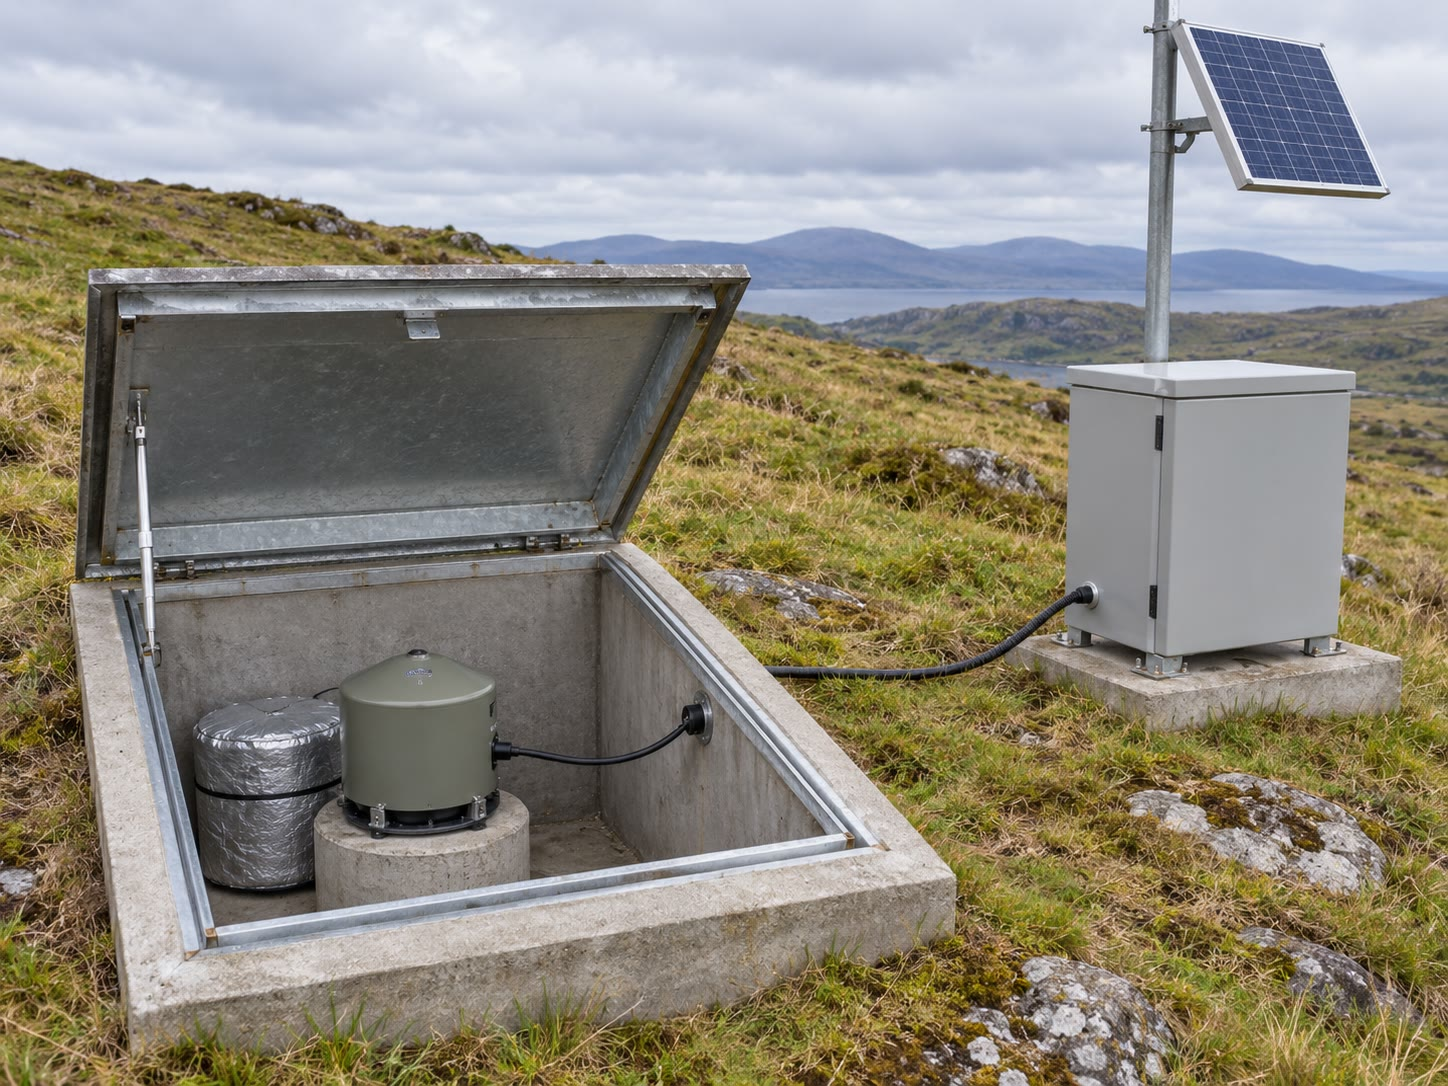
\includegraphics[width=\linewidth]{images/book5/ai/b3-seismic-vault.jpg}

{\scriptsize 宽频地震仪位于台站观测室中的墩座上
（AI 生成插图）。}
\end{minipage}
\end{inthefield}

\section{练习}

\begin{exercise}[$\star$]\label{exo:b3:seismology-imaging:1}
P 射线自地表出发（$R = \qty{6371}{km}$，$v_0 = \qty{5.80}{km.s^{-1}}$）
其\omterm{def:b3:seismology-imaging:ray-parameter}{射线参数}为 $p = \qty{500}{s.rad^{-1}}$。(a) 求其出射角；
(b) PREM 给出深度 \qty{771}{km} 处 P 波速度为 \qty{11.066}{km.s^{-1}}，
在 \qty{871}{km} 处为 \qty{11.245}{km.s^{-1}}。求两深度处的 $r/v$，
并用线性插值求该射线的转折深度。
% ledger: ak135:crust, data:prem
\end{exercise}

\begin{exercise}[$\star$]\label{exo:b3:seismology-imaging:2}
本章经 PREM 计算的 P 波走时，在 \ang{30} 处为 \qty{369.6}{s}，
在 \ang{40} 处为 \qty{455.5}{s}。(a) 估计两者之间走时曲线的斜率，
分别以 \unit{s} 每度与 \unit{s.rad^{-1}} 表示。(b) 由此推出
沿地表的波前视速度，以
\unit{km.s^{-1}} 表示。(c) 到达 \ang{35} 的射线在转折点处的 P 波速度为多少，
若其在半径 \qty{5450}{km} 处转折？
\end{exercise}

\begin{exercise}[$\star$]\label{exo:b3:seismology-imaging:3}
在本章的\omterm{def:b3:seismology-imaging:surface-waves}{勒夫波}模型中，层的 $\beta_1 =
\qty{3.5}{km.s^{-1}}$，$\rho_1 = \qty{2700}{kg.m^{-3}}$，半空间为
$\beta_2 = \qty{4.5}{km.s^{-1}}$，$\rho_2 = \qty{3300}{kg.m^{-3}}$。
(a) 求两个剪切模量。(b) 在 \qty{20}{s} 处，相速度为
\qty{3.79}{km.s^{-1}}，求波长，并将其与层厚
\qty{35}{km} 比较。(c) 已知 \qty{20}{s} 时群速度为 \qty{3.384}{km.s^{-1}}，
在 \qty{100}{s} 时为 \qty{4.333}{km.s^{-1}}，则
在 \qty{4000}{km} 外的台站，20 s 波比 100 s 波晚到多少分钟？
\end{exercise}

\begin{exercise}[$\star$]\label{exo:b3:seismology-imaging:4}
观测到的 ${}_0S_2$ 与 ${}_0T_2$ 的周期为 \qty{53.89}{min} 和
\qty{44.01}{min}。(a) 求其频率，以 \unit{mHz} 表示。(b) 地球一天内
每种各完成多少次振动？(c) 两个谱峰
只有记录时长至少为其频率差的倒数，二者才能分开。
要分开这两个简正模式，记录应持续多久？
% ledger: seis5:modes-S, seis5:modes-T
\end{exercise}

\begin{exercise}[$\star\star$]\label{exo:b3:seismology-imaging:5}
在半径为 $R$、波速均匀为 $v$ 的球体中，射线为直线弦。
(a) 证明到达 $\Delta$ 处的射线
走时为 $T = 2R\sin(\Delta/2)/v$。(b) 取 $R = \qty{6371}{km}$ 与
$v = \qty{10.0}{km.s^{-1}}$，求 \ang{30} 与 \ang{90} 处的 $T$，并与
PREM 走时 \qty{369.6}{s} 与 \qty{779.7}{s} 比较。(c) 解释为何
均匀球体在 \ang{30} 处偏快、在 \ang{90} 处偏慢。
\end{exercise}

\begin{exercise}[$\star\star$]\label{exo:b3:seismology-imaging:6}
在泊松固体（$\lambda = \mu$，故 $\alpha^2 = 3\beta^2$）中，\omterm{def:b3:seismology-imaging:surface-waves}{瑞利波}
速度 $c$ 满足，其中 $\xi = c^2/\beta^2$，
$(2 - \xi)^2 = 4\sqrt{1 - \xi/3}\,\sqrt{1 - \xi}$。(a) 将其平方并证明
其根满足 $(\xi - 4)(3\xi^2 - 12\xi + 8) = 0$。(b) 证明满足
$0 < \xi < 1$ 的唯一根为 $\xi = 2 - 2/\sqrt3$，并求 $c/\beta$。
(c) 在 ak135 上地壳中，$\beta = \qty{3.46}{km.s^{-1}}$，求
\omterm{def:b3:seismology-imaging:surface-waves}{瑞利波}速度，以及\omterm{def:b3:seismology-imaging:surface-waves}{瑞利波}在
\qty{1000}{km} 处落后于 S 波的延迟。
% ledger: ak135:crust
\end{exercise}

\begin{exercise}[$\star\star$]\label{exo:b3:seismology-imaging:7}
折射测线上四个台站的首波到时，距炮点分别为 50、100、150 和
\qty{200}{km}，到时分别为 9.0、15.3、21.5 和 \qty{27.9}{s}，误差
分别为 0.1、0.1、0.2 与 \qty{0.2}{s}。用加权最小二乘拟合 $T = a + bx$，
写出 $\mathsf G$ 与 $\mathsf C_d$，列出法方程，并
给出 $a$、$b$ 及其标准误差、速度 $1/b$ 及其误差，以及
最小 $\chi^2$。该拟合是否可接受？
\end{exercise}

\begin{exercise}[$\star\star$]\label{exo:b3:seismology-imaging:8}
一条射线穿过两个单元，长度分别为 \qty{30}{km} 和 \qty{40}{km}，
其残差为 \qty{0.50}{s}。(a) 为何 $\mathsf N = \mathsf G^{\mathsf T}
\mathsf G$ 奇异？(b) 在能精确拟合该残差的模型中，
范数最小者为 $\mathbf m = \mathsf G^{\mathsf T}(\mathsf G\mathsf
G^{\mathsf T})^{-1}\mathbf d$：求该解。(c) 计算矩阵
$\mathsf R = \mathsf G^{\mathsf T}(\mathsf G\mathsf G^{\mathsf T})^{-1}\mathsf G$
及其迹。(d) 若真实异常为 \qty{0.01}{s.km^{-1}}，且仅位于第一个
单元中，则恢复出的是什么？
\end{exercise}

\begin{exercise}[$\star\star$]\label{exo:b3:seismology-imaging:9}
地幔中一板片区域比其外界快 \qty{3}{\percent}，
其中 $v = \qty{9.0}{km.s^{-1}}$。(a) 计算竖直穿过其中 \qty{200}{km}
的射线残差，分别由\cref{prop:b3:seismology-imaging:linear}
给出的线性化公式与精确方法计算。(b) 对穿过其 \qty{100}{km} 厚度的射线，
与板片法线成 \ang{40} 夹角，同样计算其残差。(c) 线性化的相对
误差是多少？
\end{exercise}

\begin{exercise}[$\star\star\star$]\label{exo:b3:seismology-imaging:10}
在\cref{thm:b3:seismology-imaging:love}中，阶数为 $n$ 的泛频仅
在周期足够短时存在。(a) 证明在截止处其相速度为
$\beta_2$，且 $kHq_1 = n\pi$。(b) 推出截止角频率
$\omega_n = n\pi\beta_1\beta_2/\bigl(H\sqrt{\beta_2^2 - \beta_1^2}\bigr)$.
  (c) 对本章模型，计算第一泛频的截止周期
($H = \qty{35}{km}$, $\beta_1 = 3.5$, $\beta_2 = \qty{4.5}{km.s^{-1}}$).
  (d) 证明基阶模式无截止，且其相速度
  在短周期时趋于 $\beta_1$。
\end{exercise}

\begin{exercise}[$\star\star\star$]\label{exo:b3:seismology-imaging:11}
取练习 8 中的射线，数据误差取单位值。(a) 证明：对任意
$\varepsilon > 0$, $(\mathsf G^{\mathsf T}\mathsf G + \varepsilon^2\mathsf
I)^{-1}\mathsf G^{\mathsf T} = \mathsf G^{\mathsf T}(\mathsf G\mathsf
G^{\mathsf T} + \varepsilon^2\mathsf I)^{-1}$。(b) 由此推出阻尼分辨率矩阵
矩阵 $\mathsf R_\varepsilon = \mathsf G^{\mathsf T}\mathsf G/(\|\mathbf g\|^2 +
\varepsilon^2)$，其中 $\mathbf g = (30, 40)$，并求其迹。(c) 计算
迹与数据残差，取 $\varepsilon^2 = 0$、2500 与 \num{10000}
（单位为 \unit{km^2}）。描述二者的折中关系。
\end{exercise}

\begin{exercise}[$\star\star\star$]\label{exo:b3:seismology-imaging:12}
在练习 5 的均匀球体中：(a) 由
\cref{thm:b3:seismology-imaging:benndorf} 证明 $p(\Delta) = (R/v)\cos(\Delta/2)$，
并对照 $p$ 的定义（弦的出射角）检验。
(b) 证明到达 $\Delta_1$ 的射线在 $r_1 = R\cos(\Delta_1/2)$ 处转折。
(c) 在本阶段不加证明地承认 $\int_0^{\Delta_1}\operatorname{arccosh}\bigl(\cos(\Delta/2)
/\cos(\Delta_1/2)\bigr)\,\mathrm d\Delta = \pi\ln\bigl(1/\cos(\Delta_1/2)\bigr)$,
证明\omterm{prop:b3:seismology-imaging:herglotz}{赫格洛茨–维歇特反演}公式给出 $r_1$ 及速度 $v$。
\end{exercise}

\section{问题：台站 K 之下的板片}

\begin{problem}[{周末问题 --- 射线、勒夫波与
虚构台站之下的小型层析成像}]
\label{pb:b3:seismology-imaging:1}
% values: calc/ch01.py (invented station and models; Love-wave model as in the chapter)
台站 K 位于俯冲带上方的大陆上。本题
将其记录分三方面使用：地壳中的射线、\omterm{def:b3:seismology-imaging:surface-waves}{勒夫波}穿过该区域的频散，
以及其下地幔的一次小型层析成像。

\medskip
\noindent\textbf{第一部分 --- 梯度介质中的射线。}在足够短、
可略去地球曲率的距离内，K 之下的 P 波速度随深度线性增加，
$v(z) = v_0 + gz$，其中 $v_0 = \qty{5.0}{km.s^{-1}}$，且
$g = \qty{0.05}{s^{-1}}$（$z$ 以千米计）。
\begin{enumerate}
  \item 在平层中，斯涅耳定律使 $p = \sin i/v$ 保持不变。一条射线
        自 K 出发，$\sin i_0 = 0.8$：求 $i_0$ 与 $p$。
  \item 射线在何深度转折？该处速度是多少？
  \item 证明沿射线 $\mathrm di/\mathrm ds = pg$ 成立，从而它是一段
        圆弧；求其半径与圆心的深度。
  \item 计算射线回到
        地表时的水平距离 $X$。
  \item 证明 $\mathrm dT = \mathrm di/(g\sin i)$，并精确计算
        走时 $T$。
  \item 计算 $X$ 与 $T$（取 $p = \qty{0.15}{s.km^{-1}}$），并检验
        两射线之间的 $\Delta T/\Delta X$ 介于两个
        $p$ 值之间。
\end{enumerate}

\noindent\textbf{第二部分 --- \omterm{def:b3:seismology-imaging:surface-waves}{勒夫波}与地壳。}K 之下的地壳为一层
横波速度 $\beta_1 = \qty{3.5}{km.s^{-1}}$、密度
$\rho_1 = \qty{2.7}{g.cm^{-3}}$ 的层覆于地幔之上，$\beta_2 =
\qty{4.5}{km.s^{-1}}$、$\rho_2 = \qty{3.3}{g.cm^{-3}}$；其厚度 $H$ 为
未知。K 与相邻台站之间测得的\omterm{def:b3:seismology-imaging:surface-waves}{勒夫波}相速度为
周期 \qty{25}{s} 时 \qty{3.99}{km.s^{-1}}，
周期 \qty{40}{s} 时 \qty{4.25}{km.s^{-1}}。
\begin{enumerate}[resume]
  \item 计算 $\mu_1$ 与 $\mu_2$（单位 \unit{GPa}）。
  \item 在 \qty{25}{s} 处，计算 $k$、$q_1$ 与 $q_2$。
  \item 由基阶模式的频散方程求 $H$。
  \item 在 \qty{40}{s} 处同样求解。两结果是否一致？
  \item 将两周期之间的群速度估计为
        $\Delta\omega/\Delta k$，并与相速度作比较。
  \item 计算各周期的波长，并解释为何两个
        周期对地壳与最上部地幔的敏感比例
        有所不同。
\end{enumerate}

\noindent\textbf{第三部分 --- 四单元层析成像。}K 之下有一块
地幔，竖直剖面为 \qty{200}{km} × \qty{200}{km}，被切分为四
边长为 \qty{100}{km} 的方形单元：1（左上）、2（右上）、3（左下）
及 4（右下）；海沟与海洋位于左侧。参考速度为 $v_0 = \qty{8.0}{km.s^{-1}}$。在一
理想化实验中，六条直线射线穿过该块体：A 沿上排（单元 1
与 2）、B 沿下排（3 与 4）、C 沿左列（1 与 3）、D
沿右列（2 与 4）、E 沿经过 1 与 4 的对角线、F 沿
经过 2 与 3 的对角线。它们的残差为：
\begin{center}
\small
\begin{tabular}{lcccccc}
\hline
射线 & A & B & C & D & E & F \\
$\delta t$ (\unit{s}) & $0.16$ & $-0.48$ & $-0.36$ & $0.11$ & $-0.15$ & $-0.27$ \\
误差 $\sigma$ (\unit{s}) & 0.05 & 0.05 & 0.05 & 0.05 & 0.10 & 0.10 \\
\hline
\end{tabular}
\end{center}
取模型 $\mathbf m$ 为各单元的慢度扰动，以
\unit{ms.km^{-1}} 为单位（$\qty{1}{ms.km^{-1}} = \qty{e-3}{s.km^{-1}}$），使得
$\mathsf G$ 的元素等于以 \unit{km} 计的射线长度除以 1000。
\begin{enumerate}[resume]
  \item 写出 $\mathsf G$，它是一个 $6\times4$ 矩阵。
  \item 证明 $\mathsf N = \mathsf G^{\mathsf T}\mathsf C_d^{-1}\mathsf G$
        的各行分别为 $(10, 4, 4, 2)$、$(4, 10, 2, 4)$、$(4, 2, 10, 4)$、
        $(2, 4, 4, 10)$.
  \item 计算 $\mathbf b = \mathsf G^{\mathsf T}\mathsf C_d^{-1}\mathbf d$。
  \item 验证 $(1,1,1,1)$、$(1,-1,-1,1)$、$(1,1,-1,-1)$ 与 $(1,-1,1,-1)$
        均为 $\mathsf N$ 的特征向量，本征值依次为 20、4、8 与 8，并
        由此推出 $\mathsf N^{-1}$ 的各行为 $(11, -4, -4, 1)/80$、
        $(-4, 11, 1, -4)/80$、$(-4, 1, 11, -4)/80$ 与 $(1, -4, -4, 11)/80$。
  \item 计算\omterm{thm:b3:seismology-imaging:wls}{加权最小二乘估计} $\hat{\mathbf m}$。
  \item 将其换算为相对速度异常 $\delta v/v_0$，以百分数表示。
  \item 给出各单元的标准误差（分别以 \unit{ms.km^{-1}} 与百分数表示），
        以及单元 1 与 2 之间、单元 1 与
        4 之间的相关系数，并解释其符号。
  \item 计算拟合后六条射线的残差及最小
        $\chi^2$。该结果是否与给定误差相符？
\end{enumerate}

\noindent\textbf{第四部分 --- 阻尼、分辨率与板片。}
\begin{enumerate}[resume]
  \item 对于 $\varepsilon^2 = 4$（取 $\mathsf N$ 的单位），求
        $\mathsf R = (\mathsf N + 4\mathsf I)^{-1}\mathsf N$ 的本征值，并
        证明 $\mathsf R$ 的对角元为 $2/3$，共享同一行或同一列射线的单元之间为 $1/12$，
        而单元 1 与 4 之间为 $0$，
        单元 2 与 3 之间亦如此。
  \item 计算单元 3 的阻尼估计及其速度异常，并解释为何它
        小于未阻尼的结果？
  \item 阻尼模型的 $\chi^2 = 15.8$，范数为 \qty{2.91}{ms.km^{-1}}；
        未阻尼模型的 $\chi^2 = 0.50$，范数为 \qty{4.24}{ms.km^{-1}}。应保留
        哪一个？为何本题不需要阻尼？
  \item 读取阻尼 $\mathsf R$ 的第 3 行：单元 3 的估计
        被哪些单元所模糊？
  \item 哪个单元快，哪个单元慢？请从俯冲带的角度解释位于
        K 之下且靠海洋一侧的快速单元。
  \item 给出板片单元的 P 波速度异常（以百分数表示）及其
        标准误差。
\end{enumerate}
\end{problem}
